\section{Model\-Nintegrator  Class Reference}
\label{classModelNintegrator}\index{ModelNintegrator@{Model\-Nintegrator}}
The \char`\"{}nonholonomic integrator\char`\"{}, used by R. Brockett and many others. 


{\tt \#include $<$modelmisc.h$>$}

Inheritance diagram for Model\-Nintegrator::\begin{figure}[H]
\begin{center}
\leavevmode
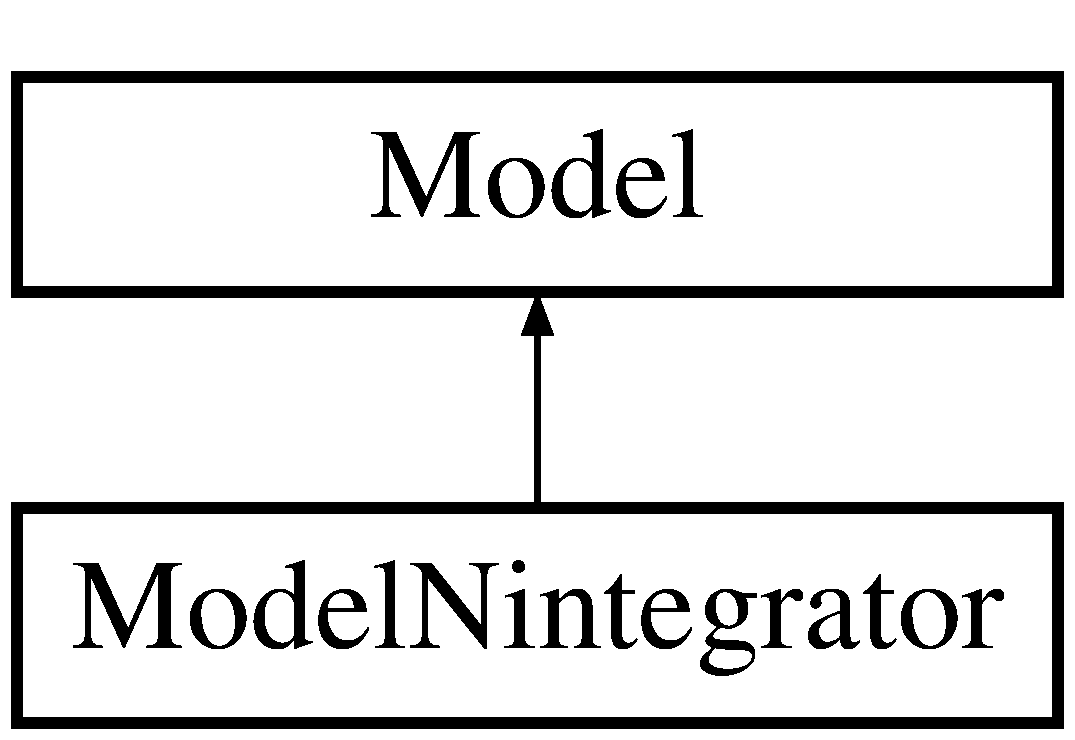
\includegraphics[height=2cm]{classModelNintegrator}
\end{center}
\end{figure}
\subsection*{Public Methods}
\begin{CompactItemize}
\item 
{\bf Model\-Nintegrator} (string path)
\item 
virtual {\bf $\sim$Model\-Nintegrator} ()
\item 
virtual {\bf MSLVector} {\bf State\-To\-Configuration} (const {\bf MSLVector} \&{\bf x})
\begin{CompactList}\small\item\em A method that converts a {\bf Model} {\rm (p.\,\pageref{classModel})} state in to a {\bf Geom} {\rm (p.\,\pageref{classGeom})} configuration.\item\end{CompactList}\item 
virtual {\bf MSLVector} {\bf Integrate} (const {\bf MSLVector} \&{\bf x}, const {\bf MSLVector} \&u, const double \&h)
\begin{CompactList}\small\item\em Perform integration from state x, using input u, over time step h.\item\end{CompactList}\item 
virtual {\bf MSLVector} {\bf State\-Transition\-Equation} (const {\bf MSLVector} \&{\bf x}, const {\bf MSLVector} \&u)
\begin{CompactList}\small\item\em The state transition equation, or equations of motion, xdot=f(x,u).\item\end{CompactList}\end{CompactItemize}
\subsection*{Public Attributes}
\begin{CompactItemize}
\item 
double {\bf UBound}
\item 
double {\bf VBound}
\end{CompactItemize}


\subsection{Detailed Description}
The \char`\"{}nonholonomic integrator\char`\"{}, used by R. Brockett and many others.



\subsection{Constructor \& Destructor Documentation}
\index{ModelNintegrator@{Model\-Nintegrator}!ModelNintegrator@{ModelNintegrator}}
\index{ModelNintegrator@{ModelNintegrator}!ModelNintegrator@{Model\-Nintegrator}}
\subsubsection{\setlength{\rightskip}{0pt plus 5cm}Model\-Nintegrator::Model\-Nintegrator (string {\em path})}\label{classModelNintegrator_a0}


\index{ModelNintegrator@{Model\-Nintegrator}!~ModelNintegrator@{$\sim$ModelNintegrator}}
\index{~ModelNintegrator@{$\sim$ModelNintegrator}!ModelNintegrator@{Model\-Nintegrator}}
\subsubsection{\setlength{\rightskip}{0pt plus 5cm}virtual Model\-Nintegrator::$\sim$Model\-Nintegrator ()\hspace{0.3cm}{\tt  [inline, virtual]}}\label{classModelNintegrator_a1}




\subsection{Member Function Documentation}
\index{ModelNintegrator@{Model\-Nintegrator}!Integrate@{Integrate}}
\index{Integrate@{Integrate}!ModelNintegrator@{Model\-Nintegrator}}
\subsubsection{\setlength{\rightskip}{0pt plus 5cm}{\bf MSLVector} Model\-Nintegrator::Integrate (const {\bf MSLVector} \& {\em x}, const {\bf MSLVector} \& {\em u}, const double \& {\em h})\hspace{0.3cm}{\tt  [virtual]}}\label{classModelNintegrator_a3}


Perform integration from state x, using input u, over time step h.



Implements {\bf Model} {\rm (p.\,\pageref{classModel_a5})}.\index{ModelNintegrator@{Model\-Nintegrator}!StateToConfiguration@{StateToConfiguration}}
\index{StateToConfiguration@{StateToConfiguration}!ModelNintegrator@{Model\-Nintegrator}}
\subsubsection{\setlength{\rightskip}{0pt plus 5cm}{\bf MSLVector} Model\-Nintegrator::State\-To\-Configuration (const {\bf MSLVector} \& {\em x})\hspace{0.3cm}{\tt  [virtual]}}\label{classModelNintegrator_a2}


A method that converts a {\bf Model} {\rm (p.\,\pageref{classModel})} state in to a {\bf Geom} {\rm (p.\,\pageref{classGeom})} configuration.



Reimplemented from {\bf Model} {\rm (p.\,\pageref{classModel_a8})}.\index{ModelNintegrator@{Model\-Nintegrator}!StateTransitionEquation@{StateTransitionEquation}}
\index{StateTransitionEquation@{StateTransitionEquation}!ModelNintegrator@{Model\-Nintegrator}}
\subsubsection{\setlength{\rightskip}{0pt plus 5cm}{\bf MSLVector} Model\-Nintegrator::State\-Transition\-Equation (const {\bf MSLVector} \& {\em x}, const {\bf MSLVector} \& {\em u})\hspace{0.3cm}{\tt  [virtual]}}\label{classModelNintegrator_a4}


The state transition equation, or equations of motion, xdot=f(x,u).



Implements {\bf Model} {\rm (p.\,\pageref{classModel_a3})}.

\subsection{Member Data Documentation}
\index{ModelNintegrator@{Model\-Nintegrator}!UBound@{UBound}}
\index{UBound@{UBound}!ModelNintegrator@{Model\-Nintegrator}}
\subsubsection{\setlength{\rightskip}{0pt plus 5cm}double Model\-Nintegrator::UBound}\label{classModelNintegrator_m0}


\index{ModelNintegrator@{Model\-Nintegrator}!VBound@{VBound}}
\index{VBound@{VBound}!ModelNintegrator@{Model\-Nintegrator}}
\subsubsection{\setlength{\rightskip}{0pt plus 5cm}double Model\-Nintegrator::VBound}\label{classModelNintegrator_m1}




The documentation for this class was generated from the following files:\begin{CompactItemize}
\item 
{\bf modelmisc.h}\item 
{\bf modelmisc.C}\end{CompactItemize}
